% Figure 1: ranking versus trustworthy numbers, told with two weather forecasters.
% Build: xelatex fig1_forecaster.tex
\documentclass[border=2pt]{standalone}
\usepackage{fontspec}
\setmainfont{Times New Roman}
\XeTeXgenerateactualtext=1   % ";" and U+037E share a glyph in Times New Roman
\XeTeXgenerateactualtext=1   % ";" and U+037E share a glyph in Times New Roman
\usepackage{tikz}
\usetikzlibrary{positioning}
\definecolor{rain}{HTML}{0072B2}
\definecolor{dry}{HTML}{B0B0B0}
\definecolor{ink}{HTML}{222222}
\definecolor{good}{HTML}{009E73}
\definecolor{bad}{HTML}{D55E00}

% one day: a filled drop (it rained) or an open circle (it stayed dry)
\newcommand{\rainday}[2]{\fill[rain] (#1,#2) circle (0.13);}
\newcommand{\dryday}[2]{\draw[dry, line width=0.8pt, fill=white] (#1,#2) circle (0.13);}

% a 0-100% scale of forecast chances, 8 cm long, at height #1
\newcommand{\scale}[1]{%
  \draw[ink, line width=0.5pt] (0,#1) -- (8,#1);
  \foreach \p in {0,20,40,60,80,100} {
    \draw[ink, line width=0.5pt] (\p*0.08,#1) -- (\p*0.08,#1-0.1);
    \node[ink, font=\footnotesize, below] at (\p*0.08,#1-0.08) {\p\%};
  }
}

\begin{document}
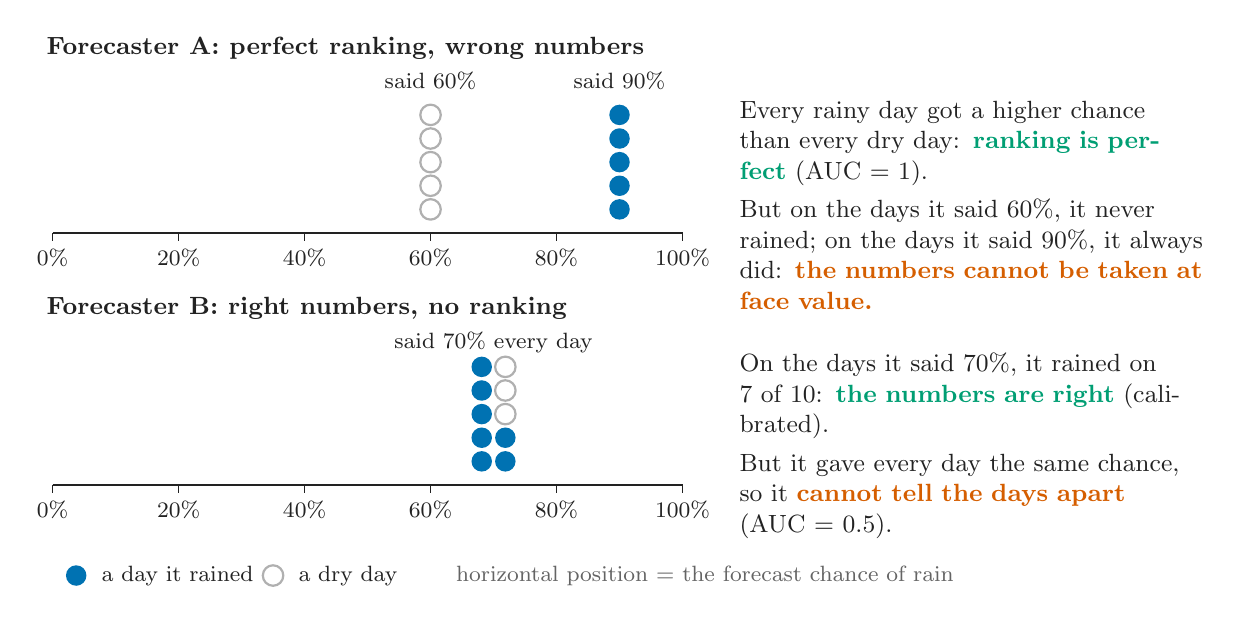
\begin{tikzpicture}[font=\small, text=ink]

% ------------------------------------------------------------- forecaster A
\node[anchor=west, font=\small\bfseries] at (-0.2,4.95) {Forecaster A: perfect ranking, wrong numbers};
\scale{2.6}
% five rainy days forecast 90%, five dry days forecast 60%
\foreach \k in {0,...,4} { \rainday{7.2}{2.9+0.3*\k} }
\foreach \k in {0,...,4} { \dryday{4.8}{2.9+0.3*\k} }
\node[font=\footnotesize, anchor=south] at (4.8,4.3) {said 60\%};
\node[font=\footnotesize, anchor=south] at (7.2,4.3) {said 90\%};
\node[anchor=north west, text width=5.9cm, align=left] at (8.6,4.4) {
  Every rainy day got a higher chance than every dry day:
  \textcolor{good}{\textbf{ranking is perfect}} \mbox{(AUC = 1)}.\\[3pt]
  But on the days it said 60\%, it never rained; on the days it said 90\%, it always did:
  \textcolor{bad}{\textbf{the numbers cannot be taken at face value.}}};

% ------------------------------------------------------------- forecaster B
\node[anchor=west, font=\small\bfseries] at (-0.2,1.65) {Forecaster B: right numbers, no ranking};
\scale{-0.6}
% ten days all forecast 70%: seven rained, three stayed dry
% two columns of five, seven of them rainy
\foreach \k in {0,...,4} { \rainday{5.45}{-0.3+0.3*\k} }
\foreach \k in {0,1} { \rainday{5.75}{-0.3+0.3*\k} }
\foreach \k in {2,3,4} { \dryday{5.75}{-0.3+0.3*\k} }
\node[font=\footnotesize, anchor=south] at (5.6,0.95) {said 70\% every day};
\node[anchor=north west, text width=5.9cm, align=left] at (8.6,1.2) {
  On the days it said 70\%, it rained on \mbox{7 of 10}:
  \textcolor{good}{\textbf{the numbers are right}} (calibrated).\\[3pt]
  But it gave every day the same chance, so it
  \textcolor{bad}{\textbf{cannot tell the days apart}} \mbox{(AUC = 0.5)}.};

% ------------------------------------------------------------- key
\rainday{0.3}{-1.75}
\node[anchor=west, font=\footnotesize] at (0.5,-1.75) {a day it rained};
\dryday{2.8}{-1.75}
\node[anchor=west, font=\footnotesize] at (3.0,-1.75) {a dry day};
\node[anchor=west, font=\footnotesize, text=ink!70] at (5.0,-1.75) {horizontal position = the forecast chance of rain};
\end{tikzpicture}
\end{document}
